\documentclass{article}
\usepackage{setspace}
\usepackage{graphicx}
\usepackage{amsmath}
\usepackage{textcomp}
\usepackage{amssymb} 
\usepackage{amsfonts}
\usepackage{amsmath}
\usepackage{amssymb}
\usepackage{amsthm}
\usepackage{esint}
\usepackage{bm}
\usepackage{tikz}
\usepackage{geometry}
\usepackage{fancyhdr}
\usepackage{siunitx}
\usepackage{wrapfig}
\usepackage{tikz}
\usetikzlibrary{fit,positioning,arrows,automata}
\usepackage{fancyhdr}
\usepackage{amsmath,amsfonts,amssymb,mathabx,stmaryrd}
\usepackage{graphicx}
\usepackage{mathptmx}
\usepackage{booktabs}
\usepackage[labelfont=bf]{caption}
\usepackage{indentfirst}
\usepackage{caption}
\usepackage{enumitem}
\usepackage{subfigure}
\usepackage{fontspec}
\usepackage{amsmath}
\newtheorem{define}{Define}[section]
\newtheorem*{theorem}{Theorem}
\newtheorem{lemma}{Lemma}[section]
\newtheorem{lemmaproof}{Lemma Proof}[section]
\newtheorem{example}{Example}[section]
% Please change the following fonts if they are not available.
\setmainfont{Times New Roman}

\addtolength{\topmargin}{-20pt}
\setlength{\oddsidemargin}{0.2cm}
\setlength{\evensidemargin}{\oddsidemargin}
\setlength{\textwidth}{15.00cm}
\setlength{\textheight}{22.50cm}
\begin{document}
\title{ \linespread{1.9}\selectfont 
Notes}
    \date{Oct 9 2019}
    \maketitle


We tend to find the Forward-backward algorithm for the new model.

Suppose we have T observations and T hidden states. Let $X_i$ denote the ith observation where $X_i\in \{ v_1, v_2, \cdots, v_k\} $ ( or just 1, $\cdots $k for convinience). Let $Z_i$ denote the ith hidden states where $Z_i\in \{ o_1, o_2, \cdots, o_m\}$ ( or just 1, $\cdots$ m for convinience). The graphical model is below.


\begin{figure}[!htb]\centering
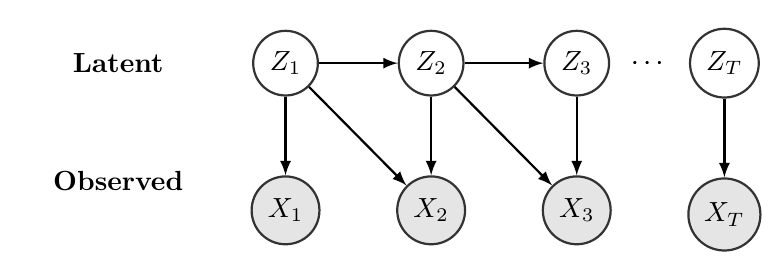
\begin{tikzpicture}
\tikzstyle{main}=[circle, minimum size = 5mm, thick, draw =black!80, node distance = 10mm]
\tikzstyle{connect}=[-latex, thick]
\tikzstyle{box}=[rectangle, draw=black!100]
  \node[box,draw=white!100] (Latent) {\textbf{Latent}};
  \node[main] (L1) [right=of Latent] {$Z_1$};
  \node[main] (L2) [right=of L1] {$Z_2$};
  \node[main] (L3) [right=of L2] {$Z_3$};
  \node[main] (Lt) [right=of L3] {$Z_T$};
  \node[box,draw=white!100] (Observed) [below=of Latent] {\textbf{Observed}};
  \node[main,fill=black!10] (O1) [right=of Observed,below=of L1] {$X_1$};
  \node[main,fill=black!10] (O2) [right=of O1,below=of L2] {$X_2$};
  \node[main,fill=black!10] (O3) [right=of O2,below=of L3] {$X_3$};
  \node[main,fill=black!10] (Ot) [right=of O3,below=of Lt] {$X_T$};
  \path (L3) -- node[auto=false]{\ldots} (Lt);
  \path (L1) edge [connect] (L2)
        (L2) edge [connect] (L3)
        (L3) -- node[auto=false]{\ldots} (Lt);
  \path (L1) edge [connect] (O1);
  \path (L2) edge [connect] (O2);
  \path (L3) edge [connect] (O3);
  \path (Lt) edge [connect] (Ot);
  \path (L1) edge [connect] (O2);
  \path (L2) edge [connect] (O3);
  \draw[dashed]  [below=of L1,above=of O1];
\end{tikzpicture}
\end{figure}

\section{Expectation Part}
Generally we need to know $P(X_{1:T})$ for future computation. From property of HMM we know
$$
P\left(X_{1 : T}, Z_{1 : T}\right)=P\left(Z_{1}\right) P\left(X_{1} | Z_{1}\right) \prod_{t=2}^{T} P\left(Z_{t} | Z_{t-1}\right)P(X_t |Z_{t-1},Z_t)
$$

Thus we repeat same operation, 

$$
\begin{aligned}
P(X_{1:T})&=\sum_{Z_{1:T}} P(X_{1:T}, Z_{1:T})\\
&=\sum_{Z_{1:T}}\underbrace{  P(Z_1)P(X_1|Z_1) }_{S_1(Z_1)}\prod_{t=2}^{T} P\left(Z_{t} | Z_{t-1}\right)P(X_t |Z_{t-1},Z_t) \\
&=\sum_{Z_{2:T}} \underbrace{\Big(  \sum_{Z_1}  S_1 P(Z_2|Z_1) P(X_2| Z_1, Z_2)\Big)}_{S_2(Z_2)} \prod_{i=3}^{T} P\left(Z_{t} | Z_{t-1}\right)P(X_t |Z_{t-1},Z_t) \\
&\cdots\\
&=\sum_{Z_{j+1:T}}\underbrace{ \Big (\sum_{Z_j}S_j P(Z_{j+1}| Z_j)P(X_{j+1}|Z_j,Z_{j+1})\Big)}_{S_{j+1}(Z_{j+1})}\prod_{t=j+2}^{T} P\left(Z_{t} | Z_{t-1}\right)P(X_t |Z_{t-1},Z_t) \\
\end{aligned}
$$

By same kind of trick, we also have
$$
\begin{aligned}
P(X_{1:T})&=\sum_{Z_{1:T}} P(X_{1:T}, Z_{1:T})\\
&=\sum_{Z_{1:T-1}}\underbrace{\sum_{Z_T} P(Z_T|Z_{T-1})P(X_T|Z_{T-1},Z_T) }_{R_{T-1}(Z_{T-1})} P(Z_1)P(X_1|Z_1) \prod_{t=2}^{T-1} P\left(Z_{t} | Z_{t-1}\right)P(X_t |Z_{t-1},Z_t) \\
&=\sum_{Z_{1:T-1}} \underbrace{\Big(  \sum_{Z_{T-1}}  R_{T-1} P(Z_{T-1}|Z_{T-2}) P(X_{T-1}| Z_{T-2}, Z_{T-1})\Big)}_{R_{T-2}(Z_{T-2})}  P(Z_1) P(X_1|Z_1)\prod_{i=2}^{T-2} P\left(Z_{t} | Z_{t-1}\right)P(X_t |Z_{t-1},Z_t) \\
&\cdots\\
&=\sum_{Z_{1:j}} \underbrace{\Big (\sum_{Z_j}R_j P(Z_{j}| Z_{j-1})P(X_{j}|Z_{j-1},Z_{j})\Big)} _{R_{j-1}(Z_{j-1})}P(Z_1)P(X_1|Z_1)  \prod_{t=2}^{j-1} P\left(Z_{t} | Z_{t-1}\right)P(X_t |Z_{t-1},Z_t) \\
\end{aligned}
$$

Thus we decomposed $P(X_{1:T})$ as function of $P(Z_{j+1}| Z_j)$, $P(X_{j+1}|Z_j, Z_{j+1})$( or $P(X_1|Z_1)$) and $P(Z_1)$ in two ways. Then we set the parameter vector $\theta$ as
\begin{itemize}
\item $\pi=( \pi_1, \cdots , \pi_m)$, where $\pi_i=P(Z_1=i)$
\item $\phi_0=\Big(b_{i n} \Big)_{m\times k}$, where $b_{in}=P(X_1=n|Z_1=i)$
\item $\phi=\big( b_{ijn} \big)_{m\times m\times k}$, where $b_{ijn}=P(X_t=n|Z_{t-1}=i,Z_t=j)$
\item $T=\Big (t_{ij}\Big)_{m\times m}$, where $t_{ij}=P(Z_{t+1}=j|Z_{t}=i)$
\item $\theta = (\pi, \phi_0, \phi, T)$
\end{itemize}

And the two notations, S and R, have specific meanings and we introduce $\alpha$ and $\beta$ here. ( If having priors $\theta$, we may condition on it).
$$
\begin{aligned}
\alpha_{t}(Z_t) := S_{t}(Z_t)&=P(X_1,\cdots, X_t,Z_t|\theta )\\
\beta_{t}(Z_t) := R_t (Z_t)&=P(X_{T},\cdots, X_{t+1}| Z_{t}, \theta)
\end{aligned}
$$

They are easy to see by checking the first term and induction relations:
$$
\begin{aligned}
\alpha_{t}(Z_t)&= \sum_{Z_{t-1}} \alpha_{t-1}P(Z_t|Z_{t-1})P(X_t|Z_{t-1}, Z_t)\\
\beta_t (Z_t)&=\sum_{Z_{t+1}} \beta_{t+1} P(Z_{t+1}|Z_t) P(X_{t+1}|Z_{t}, Z_{t+1})
\end{aligned}
$$
We also tend to find $\xi$ and $\gamma$ that
$$
\xi_t(Z_t, Z_{t+1})=P(Z_t, Z_{t+1}| X_{1:T}, \theta)
$$
$$
\gamma_t(Z_t)= P(Z_t | X_{1:T}, \theta)
$$
Clearly, $\gamma$ can be acquired by summing over $Z_{t+1}$ of $\xi$ and 
$$
\begin{aligned}
\xi_t(Z_t, Z_{t+1})=& P(Z_t, Z_{t+1}| X_{1:T}, \theta)\\
= & \frac{P(Z_t, Z_{t+1}, X_{1:T}|\theta )}{P(X_{1:T}|\theta )}\\
=& \frac{P(X_{1:t}, Z_t|\theta)P(Z_{t+1}|Z_t, \theta)P(X_{t+2:T}|Z_{t+1},\theta) P(X_{t+1}| Z_t, Z_{t+1})}{P(X_{1:T}|\theta )}\\
=&\frac{\alpha_t(Z_t) T_{Z_t, Z_{t+1}} \beta_{t+1}(Z_{t+1}) \phi(Z_t, Z_{t+1}, X_{t+1})}{\sum_{Z_t, Z_{t+1}} \alpha_t(Z_t) T_{Z_t, Z_{t+1}} \beta_{t+1}(Z_{t+1}) \phi(Z_t, Z_{t+1}, X_{t+1})}
\end{aligned}
$$
\section{Maximization Part}
Then we will use these terms for Baum-Welch algorithm. Recall that
$$
Q\left(\theta, \theta_{k}\right)=\mathbb{E}_{\theta_{k}}\left(\log p(X, Z| \theta) | X\right)
$$
thus followed by
$$
\begin{aligned} \log P(X,Z | \theta )=& \log p\left(Z_{1}|\theta \right)+\sum_{t=1}^{T-1} \log p\left(Z_{t+1} | Z_{t}, \theta \right)+ \log p( X_1| Z_1,\theta )+\sum_{t=1}^{T-1} \log p\left(X_{t+1} | Z_{t+1}, Z_{t}, \theta \right) \\=& \sum_{i=1}^{m} 1\left(Z_{1}=i\right) \log \pi_{i}+\sum_{t=1}^{T-1} \sum_{i=1}^{m} \sum_{j=1}^{m} 1\left(Z_{t}=i, Z_{t+1}=j\right) \log T_{i j} \\ &+ \sum _{i=1}^{m} 1(Z_1=i)\log{\phi_0(i, X_1)} +\sum_{t=1}^{T-1} \sum_{i=1}^{m} \sum_{j=1}^{m} 1\left(Z_{t}=i, Z_{t+1}=j\right) \log \phi _{ij}( X_{t+1}) \end{aligned}
$$
Expectation of indicator is just probability of condition in it, thus
$$
\begin{aligned}
Q\left(\theta, \theta_{k}\right)=& \sum_{i=1}^{m} P_{\theta_k}\left(Z_{1}=i | X\right) \log \pi_{i}+\sum_{t=1}^{T-1} \sum_{i=1}^{m} \sum_{j=1}^{m} P_{\theta_k}\left(Z_{t}=i, Z_{t+1}=j | X\right) \log T_{i j} \\ &+ \sum _{i=1}^{m} P_{\theta_k}(Z_1=i | X)\log{\phi_0(i, X_1)} +\sum_{t=1}^{T-1} \sum_{i=1}^{m} \sum_{j=1}^{m} P_{\theta_k}\left(Z_{t}=i, Z_{t+1}=j | X \right) \log \phi _{ij}( X_{t+1}) 
\end{aligned}
$$
And by out definition, this is
$$
Q\left(\theta, \theta_{k}\right)=\sum_{i=1}^{m} \gamma_{1 i} \log \pi_{i}\phi_0(i, X_1)+\sum_{t=1}^{T-1} \sum_{i, j=1}^{m} \xi_{t i j} \log T_{i j}+\sum_{t=1}^{T-1} \sum_{i,j =1}^{m} \xi_{t i j}\log \phi _{ij}( X_{t+1}) 
$$ 
By method of Lagrangian multipliers, we have 
$$
\begin{aligned}
\hat{\pi_{i}}=&\frac{\gamma_{1 i}}{\sum_{j=1}^{m} \gamma_{1 j}}=\gamma_{1i}\\
\hat{T_{i j}}=&\frac{\sum_{t=1}^{T-1} \xi_{t i j}}{\sum_{t=1}^{T-1} \sum_{j=1}^{m} \xi_{t i j}}=\frac{\sum_{t=1}^{T-1} \xi_{t i j}}{\sum_{t=1}^{T-1} \gamma_{t i}}\\
\hat{\phi_{0in}}= & \left\{
\begin{aligned}
1& &n=X_1 \\
0& &otherwise 
\end{aligned}
\right.\\
\hat{\phi_{ijn}}=&\frac{\sum_{X_{t+1}=n} \xi_{ijt}}{\sum_{t=1}^{T-1} \xi_{ijt}}
\end{aligned}
$$
Notice that optimization of $\phi_0$ is rather simple, we can solve this by using multiple input.

\section{Multiple Observation}

When we have multiple observations, we tend to average them in some sense to get better approximation. We consider different way of optimizing following
$$
\begin{aligned}
\pi_{i}&=P\left(Z_{1}=i\right)\\
b_{0i n}&=P\left(X_{1}=n | Z_{1}=i\right)\\
b_{i j n}&=P\left(X_{t}=n | Z_{t-1}=i, Z_{t}=j\right)\\
t_{i j}&=P\left(Z_{t+1}=j | Z_{t}=i\right)
\end{aligned}
$$
For multiple input, we have 
$$
\begin{aligned} P(X | \theta) &=\prod_{k=1}^{K} P\left(X^{k} | \theta \right) \\ &=\prod_{k=1}^{K} P_{k} \end{aligned}
$$
Since observations are independent, we have following result and by maximizing every single $P_k$, we get our multiple input approximation.
$$
\begin{aligned}
t_{i j}&=P\left(Z_{t+1}=j | Z_{t}=i, (X^1, \cdots, X^K)\right)\\
&=\frac{P\left(Z_{t+1}=j  , Z_{t}=i |(X^1, \cdots, X^K)\right)}{P(Z_t=i | (X^1, \cdots, X^K) )}\\
&=\frac{\sum_j P\left(Z_{t+1}=j  , Z_{t}=i | X^j)P(X_j| (X^1, \cdots, X^K)\right)}{\sum_j P(Z_t=i | X_j)P(X^j| (X^1, \cdots, X^K) )}\\
&=\frac{\frac{1}{K} \sum_j P(Z_{t+1}=j  , Z_{t}=i | X^j)}{\frac{1}{K} \sum_j P(Z_t=i | X^j)}\\
&=\frac{ \sum_j P(Z_{t+1}=j  , Z_{t}=i ,X^j) /P(X^j)}{ \sum_j P(Z_t=i ,X^j) /P(X^j)}
\end{aligned}
$$

Thus 
$$
\bar{t}_{i j}=\frac{\sum_{k=1}^{K} \frac{1}{P_{k}} \sum_{t=1}^{T_{k}-1} \alpha_{t}^{k}(i) t_{i j} b_{ij}\left(Z_{t+1}^{(k)}\right) \beta_{j}^{k}(Z_{t+1})}{\sum_{k=1}^{K} \frac{1}{P_{k}} \sum_{t=1}^{T_{k}-1} \alpha_{t}^{k}(i) \beta_{t}^{k}(i)}
$$
and by same way
$$
\begin{aligned}
\overline{b_{ijn}}&=\frac{\sum_{k=1}^{K} \frac{1}{P_{k}} \sum_{X_{t+1}=n}\alpha_{t}^{k}(i) \beta_{t+1}^{k}(j)}{\sum_{k=1}^{K} \frac{1}{P_{k}} \sum_{t=1}^{T_{k}-1} \alpha_{t}^{k}(i) \beta_{t+1}^{k}(j)}\\
b_{0in}&=\frac{\sum_{X^k=n} 1}{K}\\
\pi_i&=\frac{\sum_k \pi^k_i}{K}
\end{aligned}
$$

\end{document}